\documentclass[11pt]{article}

\usepackage{amsmath}
\usepackage{minted}
\usepackage{hyperref}
\usepackage[margin=2.0cm]{geometry}

\usepackage{graphicx}
\graphicspath{ {/home/ubuntu/www/octopress/source/} }

\def\title{Accelerating Options Pricing via Fourier Transforms}
\newcommand{\Rev}{\text{rev}\;}
\newcommand\del[1]{\left(#1\right)}
\newcommand\nicefrac[2]{\frac{#1}{#2}}
\newcommand\set[1]{\left\{#1\right\}}
\newcommand\cF{\mathcal{F}}
\newcommand\Asterisk{*}

\setlength\parindent{1cm}

\begin{document}

In the \href{http://andrew.gibiansky.com/blog/economics/binomial-options-pricing-model}{previous post}, I
introduced stock options and an algorithm for pricing them known as the
Binomial Options Pricing Model. However, as we saw from a simple Python
implementation, the computations for this algorithm are expensive, and it takes
$O(N^2)$ operations to compute the options price for $N$ timesteps away from
expiration. However, it turns out there is a very clever way to accelerate this
algorithm using the dicrete Fourier transform.

\section*{Discrete Fourier Transforms}
Before using discrete Fourier transforms to accelerate the Binomial Options Pricing Model algorithm,
we will first take some time to establish the definitions of the Fourier transform, its inverse, and
several other useful mathematical tools. Begin by considering a sequence of values $x_0, x_1,
\ldots, x_{n-1}$. In that case, we define the discrete Fourier transform (DFT) as a sequence $X_0, X_1,
\ldots, X_{n-1}$ where
\[X_k = \frac{1}{\sqrt{n}} \sum_{j=0}^{n-1} x_j e^{i\frac{2\pi}{n} jk}.\]
We often write the Fourier transform of a sequence as $X = \mathcal{F}(x)$. 

This equation can be understood in several ways. For instance, if you consider that the exponentials
are simply basis vectors for the vector space of functions, the Fourier transform immediately
reduces to simply a projection of the sequence $\set{x_j}$ onto the vector space, since each product
$x_j e^{i\frac{2\pi}{n} jk}$ is simply the projection onto a single basis vector. The Fourier
transform can also be viewed as a matrix multiplication, since it is simply a linear transformation
from the vector of $x_j$ observations into the frequency observations $X_k$. 

Viewing the Fourier transform as a linear transformation (via a matrix multiplication by the $\vec
x$ vector) explains the scaling factor of $\nicefrac{1}{\sqrt{n}}$, because that is the scaling
factor necessary to make the Fourier matrix a unitary transformation. Unitary matrices have the
incredibly useful property that for a unitary matrix $A$, the inverse $A^{-1}$ is equal to the
adjoint operator (conjugate transpose) $A^*$. With this in mind, we can define the inverse Fourier
transform easily by noting that the Fourier transform is symmetric and thus the conjugate transpose
is simply the conjugate of each term, and thus we simply need to change the sign in the exponential.
Thus, we obtain the expression
\[x_k = \frac{1}{\sqrt{n}} \sum_{j=0}^{n-1} X_j e^{-i\frac{2\pi}{n} jk}.\]
The inverse discrete Fourier transform is often written as $x = \mathcal{F}^{-1}(X)$.

Note that there is a very clear relationship between the Fourier transform and the inverse Fourier
transform. Consider the vector defined by the complex number $e^{i\theta} = \cos\theta +
i\sin\theta$. As $\theta$ increases, this vector traces out the unit circle, rotating around it.
Since the exponentials can be viewed as unit vectors rotating along a circle, the Fourier transform
and the inverse transform really only differ in that one of them has exponentials rotating in the
counter clockwise direction ($e^{-i\theta}$) while the other has them rotating in the clockwise
direction ($e^{i\theta}$). Thus, they only differ by which elements of the sequence get multiplied
by which exponentials. In the Fourier transform, the elements are chosen ``counter-clockwise'',
while in the inverse Fourier transform, the elements are chosen ``clockwise''. Mathematically
speaking, we can define a reversal operation 
\[\text{rev}(a_0, a_1, a_2, \ldots, a_{n-1}) = (a_0, a_{n-1}, a_{n-2}, \ldots, a_1).\]

Note that this is not a simple reversal of the elements, since the first element $a_0$ stays in the
same place. Instead, this can be viewed as a reversal of direction, with the original sequence going
``counter clockwise'' and the reversal going ``clockwise''.

\begin{center}
    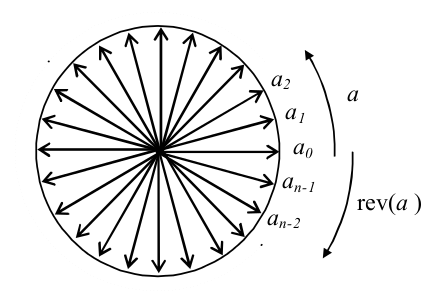
\includegraphics[scale=0.7]{images/reversal.png}
\end{center}

With this in mind, it is intuitively clear that since in the forward transform the exponentials are
rotating counter clockwise and in the inverse transform the exponentials are rotating clockwise, the
Fourier transform of a sequence will be equal to the inverse Fourier transform of the reversal:
\begin{align*}
    \mathcal{F}(x) &= \mathcal{F}^{-1}(\text{rev}(x)) \\
    \mathcal{F}^{-1}(x) &= \mathcal{F}(\text{rev}(x))
\end{align*}

\section*{Discrete Convolutions}
Now that we have established the theory behind the Discrete Fourier Transform, let us define yet
another mathematical construct known as the discrete convolution. The discrete convolution of two
$n$-dimensional vectors $a$ and $b$ with components $a_i$ and $b_i$ is a vector with components
\[\del{a \Asterisk b}_j = \sum_{i=0}^{n-1} a_{j-i} b_i\]
where if $j - i < 0$ use instead the value $j - i \mod n$. This can be viewed as aligning the two
sequences with one going in the opposite direction and starting at an offset of $j$, doing a
pointwise multiplication, and then summing up the results and letting that be the $j$th component of
the convolution.

Although this construct may seem esoteric, it turns out it is immensely useful because of the
relation that convolution holds to the Fourier transform. Consider the $k$th component of the
Fourier transform of $a \Asterisk b$:
\[
    \mathcal{F}(a \Asterisk b)_k = \frac{1}{\sqrt{n}} \sum_{j=0}^{n-1} \omega_{-kj} (a \Asterisk b)_j,
\]
where we write the exponential $\omega_x = e^{i\frac{2\pi}{n}x}$ for convenience. Expanding this
via the definition of the discrete convolution, we find that
\begin{align*}
    \mathcal{F}(a \Asterisk b)_k &= \frac{1}{\sqrt{n}} \sum_{j=0}^{n-1} \omega_{-kj} \sum_{i=0}^{n-1} a_{j-i} b_i \\
\end{align*}
We know that since exponents add during multiplication, 
\[\omega_{-kj} = e^{-i\frac{2\pi}{n}kj} = e^{-i\frac{2\pi}{n}k(j-i)} e^{-i\frac{2\pi}{n}ki} = \omega_{-k(j-i)}\omega_{-ki}\]

Using this fact in addition to the fact that the summation can be moved (due to the distributive
property), we can rewrite our Fourier transform component as
\begin{align*}
    \mathcal{F}(a \Asterisk b)_k &= \frac{1}{\sqrt{n}} \sum_{j=0}^{n-1}  \del{\omega_{-k(j-i)}\omega_{-ki}} \sum_{i=0}^{n-1} a_{j-i} b_i \\
    &= \frac{1}{\sqrt{n}} \sum_{j=0}^{n-1}\sum_{i=0}^{n-1} \omega_{-k(j-i)}\omega_{-ki} a_{j-i} b_i \\
    &= \frac{1}{\sqrt{n}} \sum_{j=0}^{n-1}\sum_{i=0}^{n-1} \del{\omega_{-k(j-i)}a_{j-i}} \del{\omega_{-ki}  b_i}
\end{align*}

If we let $m = j-l$, we can note that $m$ goes from zero to $n-1$ independently, and thus we can
rearrange the sums again to yield our final result that
\begin{align*}
    \mathcal{F}(a \Asterisk b)_k &= \frac{1}{\sqrt{n}} \del{\sum_{i=0}^{n-1} \omega_{-km}a_m} \del{\sum_{j=0}^{n-1}\omega_{-ki}  b_i} \\
    &= \sqrt{n}  \del{\frac{1}{\sqrt{n}}\sum_{i=0}^{n-1} \omega_{-km}a_m} \del{\frac{1}{\sqrt{n}}\sum_{j=0}^{n-1}\omega_{-ki}  b_i}
\end{align*}

In other words, the Fourier transform of a convolution is the scaled product of the Fourier
transforms of the vectors being convoluted:
\[\mathcal{F}(a \Asterisk b)_k = \sqrt{n}  \mathcal{F}(a)_k\mathcal{F}(b)_k\]

This property is absolutely essential to our use of the Fourier transform. Note that element-wise
multiplication of two vectors in the Fourier domain is \emph{much} faster than computing the
convolution; while we only need $N$ multiplications to compute the element-wise product,  computing
the convolution the regular way would require $N$ multiplications and a sum for \emph{each}
component, and since there are $N$ components, there would be $N^2$ multiplications. In algorithmic
terms, the element-wise multiplication is bounded from above by $O(N)$, while the convolution is
bounded by $O(N^2)$. 

The only problem is that the computation via the Fourier transform requires us to compute the
Fourier transform first; we will discuss the efficiency of computing the Fourier transform in the
last section. Although the na\"{\i}ve algorithm for computing the discrete Fourier transform turns
out to be $O(N^2)$, there are some tricks we can utilize - known together as the Fast Fourier
Transform (FFT) - which will permit us to compute the transform in $O(N\lg N)$ time instead.
\pagebreak

\section*{Accelerating the Binomial Model}
In this section, we will demonstrate that the Binomial Options Pricing Model algorithm described in
the first section can be accelerated dramatically by utilizing the Discrete Fourier Transform.
First, consider the option prices calculated for a time $t = k\Delta t$ in the future. As discussed
in the first section, this is a $k+1$-dimensional vector, which we will call $\vec C_j$. Recall that
in order to compute the first element of the vector $\vec C_{j-1}$ for the previous timestep, we
must compute the expression
\[C_{j-1, 1} = e^{-r\Delta t}\del{pC_{j, 1} + (1-p)C_{j, 2}}\]
where notationally $C_{a, b}$ is the $b$th component of the vector for time $t=a\Delta t$. More
generally, to compute $C_{j-1, k}$, we must evaluate
\[C_{j-1, k} = e^{-r\Delta t}\del{pC_{j, k} + (1-p)C_{j, k+1}}.\]
Due to the commutative property of multiplication, we can add in some zeros to this sum and rewrite
this as
\begin{align*}
C_{j-1, k} &= e^{-r\Delta t}\del{C_{j, k}p + C_{j, k+1}(1-p)} \\
=\;& e^{-r\Delta t}\del{C_{j, k}p + C_{j, k+1}(1-p) + C_{j, k+2}\cdot 0 + \cdots}.
\end{align*}
However, if we define a vector $\vec q = (p, 1-p, 0, \ldots)$ containing the growth and decay
probabilities and padded with as many zeros as necessary to make it an $n$-dimensional vector, then
we see that the above expression simply reduces to the discrete convolution
\[C_{j-1} = e^{-r\Delta t} \del{C_j \Asterisk \Rev(q)} = C_j \Asterisk \del{e^{-r\Delta t}\Rev(q)}.\]
By adding the extra padding components, we have make it so that every vector is of dimension $N+1$,
since that is the dimension of the leaf vector $C_N$.  However, only the first $j$ components
interest us, and the others are irrelevant.  Extrapolating the preceeding expression from the leaf
vector $C_N$ to the time $t=k\Delta t$, this yields the expression
\[C_k = C_N \Asterisk \underbrace{e^{-r\Delta t}\Rev(q) \Asterisk e^{-r\Delta t} \cdots \Asterisk e^{-r\Delta t}\Rev(q)}_\text{N-k times}.\]
Taking the inverse Fourier transform of both sides of the equation, we find that
\[\cF^{-1}(C_k) = \cF^{-1}(C_N) \del{\sqrt{N + 1}e^{-r\Delta t} \cF^{-1}(\Rev q)}^{N-k}\]
However, recall that $\cF^{-1}(\Rev a) = \cF(a)$, so this just becomes 
\[\cF^{-1}(C_k) = \cF^{-1}(C_N) \del{\sqrt{N + 1}e^{-r\Delta t} \cF(q)}^{N-k},\]
where the exponentiation is just repeated element-wise multiplication of the vector components. With
this equation in mind, we can compute the price of the option at time $t=0$ by substituting for
$k=0$ and taking the Fourier transform of both sides to obtain
\[C_0 = \cF\del{\cF^{-1}(C_N) \del{\sqrt{N + 1}e^{-r\Delta t} \cF(q)}^N}.\]
Since $\cF$ and $\cF^{-1}$ play symmetric roles, we could also have written this as
\[C_0 = \cF^{-1}\del{\cF(C_N) \del{\sqrt{N + 1}e^{-r\Delta t} \cF^{-1}(q)}^N}.\]

Although this result is certainly interesting and impressive, it may not be immediately obvious why
this is crucial and how this speeds up the computation of the options price. Suppose that computing
the Fourier transform or inverse Fourier transform of an $N$-length sequence takes at most some time
$f(N)$. For this algorithm, we must compute the transform of $q$ and the transform of $C_N$, and at
the end compute the inverse transform of the entire expression above, so we will ultimately spend
$3f(N)$ units of time computing Fourier transforms. In addition, we will need to raise the
components of $\cF(q)$ to the $N$th power, which is a constant time operation for each component,
and will thus take $cN$ time (since we need to do it for each of the $N$ components). Thus, the
total time spent will be $cN + 3f(N)$; therefore, if we can devise some way to compute the Fourier
transform faster than $O(N^2)$, we will have an algorithm that is provably faster than the na\"{\i}ve
Binomial Options Pricing Model and even the optimized dynamic programming algorithm (which runs in
$O(N^2)$). Luckily, algorithms for computing the discrete Fourier transforms have been well studied,
and there exists an algorithm known as the Fast Fourier Transform (FFT) which can compute the
transform in time upper bounded by $O(N \lg N)$.

\section*{Fast Fourier Transforms}

Due to the importance of the discrete Fourier transform algorithm, many different fast Fourier
transform algorithms have been developed over the years. I would like to demonstrate a single
relatively simple algorithm known as the Cooley-Tukey radix-2 algorithm, simply to demonstrate that
the discrete Fourier transform \emph{can} be computed efficiently. For the simple version of this
algorithm, we must assume that the length of the sequence $N$ is equal to some power of two;
however, although this is a significant obstacle, there are several ways to overcome it described
extensively in the literature (which we will not describe).

Suppose that you have a sequence $x_k$. Recall that the discrete Fourier transform is defined as
\[X_k = \frac{1}{\sqrt{n}} \sum_{j=0}^{n-1} x_j e^{i\frac{2\pi}{n} jk}.\]
Now, consider the two subsequences $x_{2k}$ and $x_{2k+1}$ corresponding to the even and odd terms
in the sequence. We can then define the two Fourier transforms $X_{2k} = \cF(x_{2k})$ and $X_{2k+1}
= \cF(x_{2k+1})$. Suppose that the length of those subsequences is $M=\nicefrac{N}{2}$. Assuming we
have the values of these two transforms defined by
\begin{align*}
    E_k = X_{2k} &= \frac{1}{\sqrt{n}} \sum_{j=0}^{M-1} x_{2j} e^{i\frac{2\pi}{n} jk} \\
    O_k = X_{2k+1} &= \frac{1}{\sqrt{n}} \sum_{j=0}^{M-1} x_{2j+1} e^{i\frac{2\pi}{n} jk}
\end{align*}
we can manipulate the terms of $X_k$ and show that
\[
    X_k = \begin{cases}
        E_k + e^{-i\frac{2\pi}{N}k}O_k & \text{\ if } k < M \\
        E_{k-M} - e^{-i\frac{2\pi}{N}\del{k-M}}O_{k-M} & \text{\ if } k \ge M \\
    \end{cases}
\]
Therefore, we have shown that we can take a sequence of length $N$ and express its Fourier transform
as a function of two Fourier transforms of length $\nicefrac{N}{2}$. In addition, it is clear that
for small enough sequences (say, $N=3$), the amount of time necessary to compute the discrete
Fourier transform via the original formula is negligible and can be assumed to be constant; this
small case will form the base case for recursion. We will now verify that this algorithm is
efficient by computing the running time.

This algorithm can be broken down into several steps, as follows:
\begin{enumerate}
    \item
        Given the original sequence $x_k$, examine its length $N$. 
    \item If $N$ is less than some specified small threshold, such as three, compute the
        Fourier transform via the na\"{\i}ve approach (by just computing the sums for each
        component).  Then, return the Fourier transformed sequence and do not continue the
        algorithm.
    \item If $N$ is large, separate $x_k$ into two sequences that contain the even terms
        ($x_{2k}$) and the odd terms ($x_{2k+1}$).
    \item
        Recursively compute the discrete Fourier transform of each of those sequences.
    \item
        Compute the total Fourier transform via the piecewise equation above. Return the Fourier
        transformed sequence.
\end{enumerate}

Each of these steps can be analyzed in order to determine the amount of time they take. The first
step, computing the length, takes a constant amount of time, since the data is stored in an array of
known length. The second step will either take a constant amount of time (if we're computing the
transform for a small sequence), or will take no time at all if we skip it. The third step will take
an amount of time proportional to the size of the sequence, since we must iterate over the sequence
and place each element into a new array. The last step will also take a time proportional to the
size of the sequence, since we must compute a simple mathematical expression which takes constant
time for every element in the sequence. Thus, we have found that the total time necessary for all
the steps excluding the recursion is linear in the sequence, and thus each recursion incurs $O(N)$
overhead.
\pagebreak

\onecolumn
\vspace*{0cm}

\begin{center}

\textbf{Binomial Options Pricing Model: Fast Fourier Transform Accelerated} \href{http://andrew.gibiansky.com/downloads/code/bopm\_fft.py}{(download)}

\begin{minted}{python}
#!/usr/bin/env python
from math import exp
from numpy import array
from numpy.fft import fft, ifft

# Input stock parameters
dt = input("Enter the timestep: ")
S = input("Enter the initial asset price: ")
r = input("Enter the risk-free discount rate: ")
K = input("Enter the option strike price: ")
p = input("Enter the asset growth probability p: ")
u = input("Enter the asset growth factor u: ")
N = input("Enter the number of timesteps until expiration: ")

# Input whether this is a call or a put option
call = raw_input("Is this a call or put option? (C/P) ").upper().startswith("C")

def price(k, us):
    """ Compute the stock price after 'us' growths and 'k - us' decays. """
    return S * (u ** (2 * us - k))

def leaves(k):
    """ Compute the leaves of the tree for a depth of k timesteps. """
    values = []
    for i in xrange(k + 1):
        if call: values.append(max(0, price(k, i) - K))
        else:    values.append(max(0, K - price(k, i)))
    return values

def bopm(k):
    """
    Compute the option price for an option expiring in 'k' timesteps.
    """
    # Obtain the leaf prices as a NumPy array and create the $q$ vector
    leafValues = array(list(reversed(leaves(k))))
    q = array([p, 1-p] + [0] * (k - 1))

    # Compute the options price via the fast Fourier transform
    C = ifft(fft(leafValues) * ((k + 1) * exp(-r * dt) * ifft(q)) ** k)

    # Return the first component, which is the only important one
    return C[0]

print 'Computed option price: $%.2f' % bopm(N).real
    \end{minted}
\end{center}
\newpage

In order to compute the total running time, imagine the computation tree generated by this
algorithm. The top level of the tree incurs $N$ work. The next level of the tree has two nodes
and each one incurs $N/2$ work, so in total they incur $N$ work. The next level has four nodes, each
of which incurs $N/4$ work, so once more the total at that level is $N$ overhead. Since each next
level reduces the sequence lengths by a factor of two, there must be no more than $\lg N$ levels,
and thus the total amount of work is bounded by the number of levels times the overhead at each
level, which is $O(N \lg N)$. Thus, we have shown that the discrete Fourier transform can be
computed quickly in $O(N \lg N)$ time. Recall that at the end of the previous section we
showed that if the fast Fourier transform worked in $O(N \lg N)$ time, then we could compute the
Binomial Options Pricing Model options price in $O(N \lg N)$ time, which is much faster than the
original $O(N^2)$ approach.

\section*{Conclusion}
In these two blog posts, we derived the Binomial Options Pricing Model, an alternative to the commonly used
Black-Scholes model for computing option prices. The binomial model is superior to Black-Scholes
because it allows for the possibility of exercising the option prematurely, thus allowing for
computing prices of American and Bermudan style options in addition to European style options.
However, the computational complexity of the binomial model is a significant disadvantage,
especially since the complexity grows quickly as the time until the option expiration date
increases. We define several mathematical tools such as discrete Fourier transforms and discrete
convolutions, which we then use to rederive the binomial model using Fourier transforms. Finally, we
implemented both the na\"{\i}ve $O(2^N)$ algorithm (which can be accelerated to $O(N^2)$ with
dynamic programming) and the Fourier transform based $O(N \lg N)$ algorithm, and verified that they
gave the same results for the same inputs. Thus, the use of Fourier transforms significantly
increases the applicability of the binomial options pricing model, as it speeds up the algorithm by
a factor of $\frac{N}{\lg N}$, allowing accurate pricing of American style options at high speeds.

\end{document}
